\section{Auswertung}
\label{sec:Auswertung}

Wie in \autoref{sec:Durchführung} beschrieben wird zunächst bei einer Chiptemperatur von $\qty{50}{\degreeCelsius}$, was laut vorhandener Umrechnungstabelle einer Spannung von 
$\qty{1.312}{\volt}$ am Thermoresistor entspricht, nach der Schwellenspannung ab der Laseraktivität stattfindet gesucht. Mit Hilfe der Kamera ist auf der IR-Sichtkarte deutlich zu sehen, wenn
die Diode in die Laserphase wechselt. Auf dem Monitor sieht dies dann wie in \autoref{fig:lasingphase} aus. Bei drehen des oberen Knopfes am Laser ist nun deutlich zu erkennen, wie der Laser durch
seine Moden durchwechselt. Dabei wechselt sich starke mit schwacher Intensität bzw. die Lasingaktivität mit der Diodenaktivität ab. Nach mehrmaligem Justieren sind $7$ Maxima zu erkennen, die 
der Laser bei Drehen des Knopfes durchlief. Dies ist die geringste erreichte Anzahl an Maxima. Also wird das vierte zu erkennene Maximum für die Weiterarbeit gewählt, da dieses der Logik folgend 
die größte Intnesität hat. Die Schwellenspannung an der Diode wurde dabei auf $U_{\mathrm{Schwelle}}=\qty{3.60(0.01)}{\volt}$ bestimmt. 

\begin{figure}
  \centering
  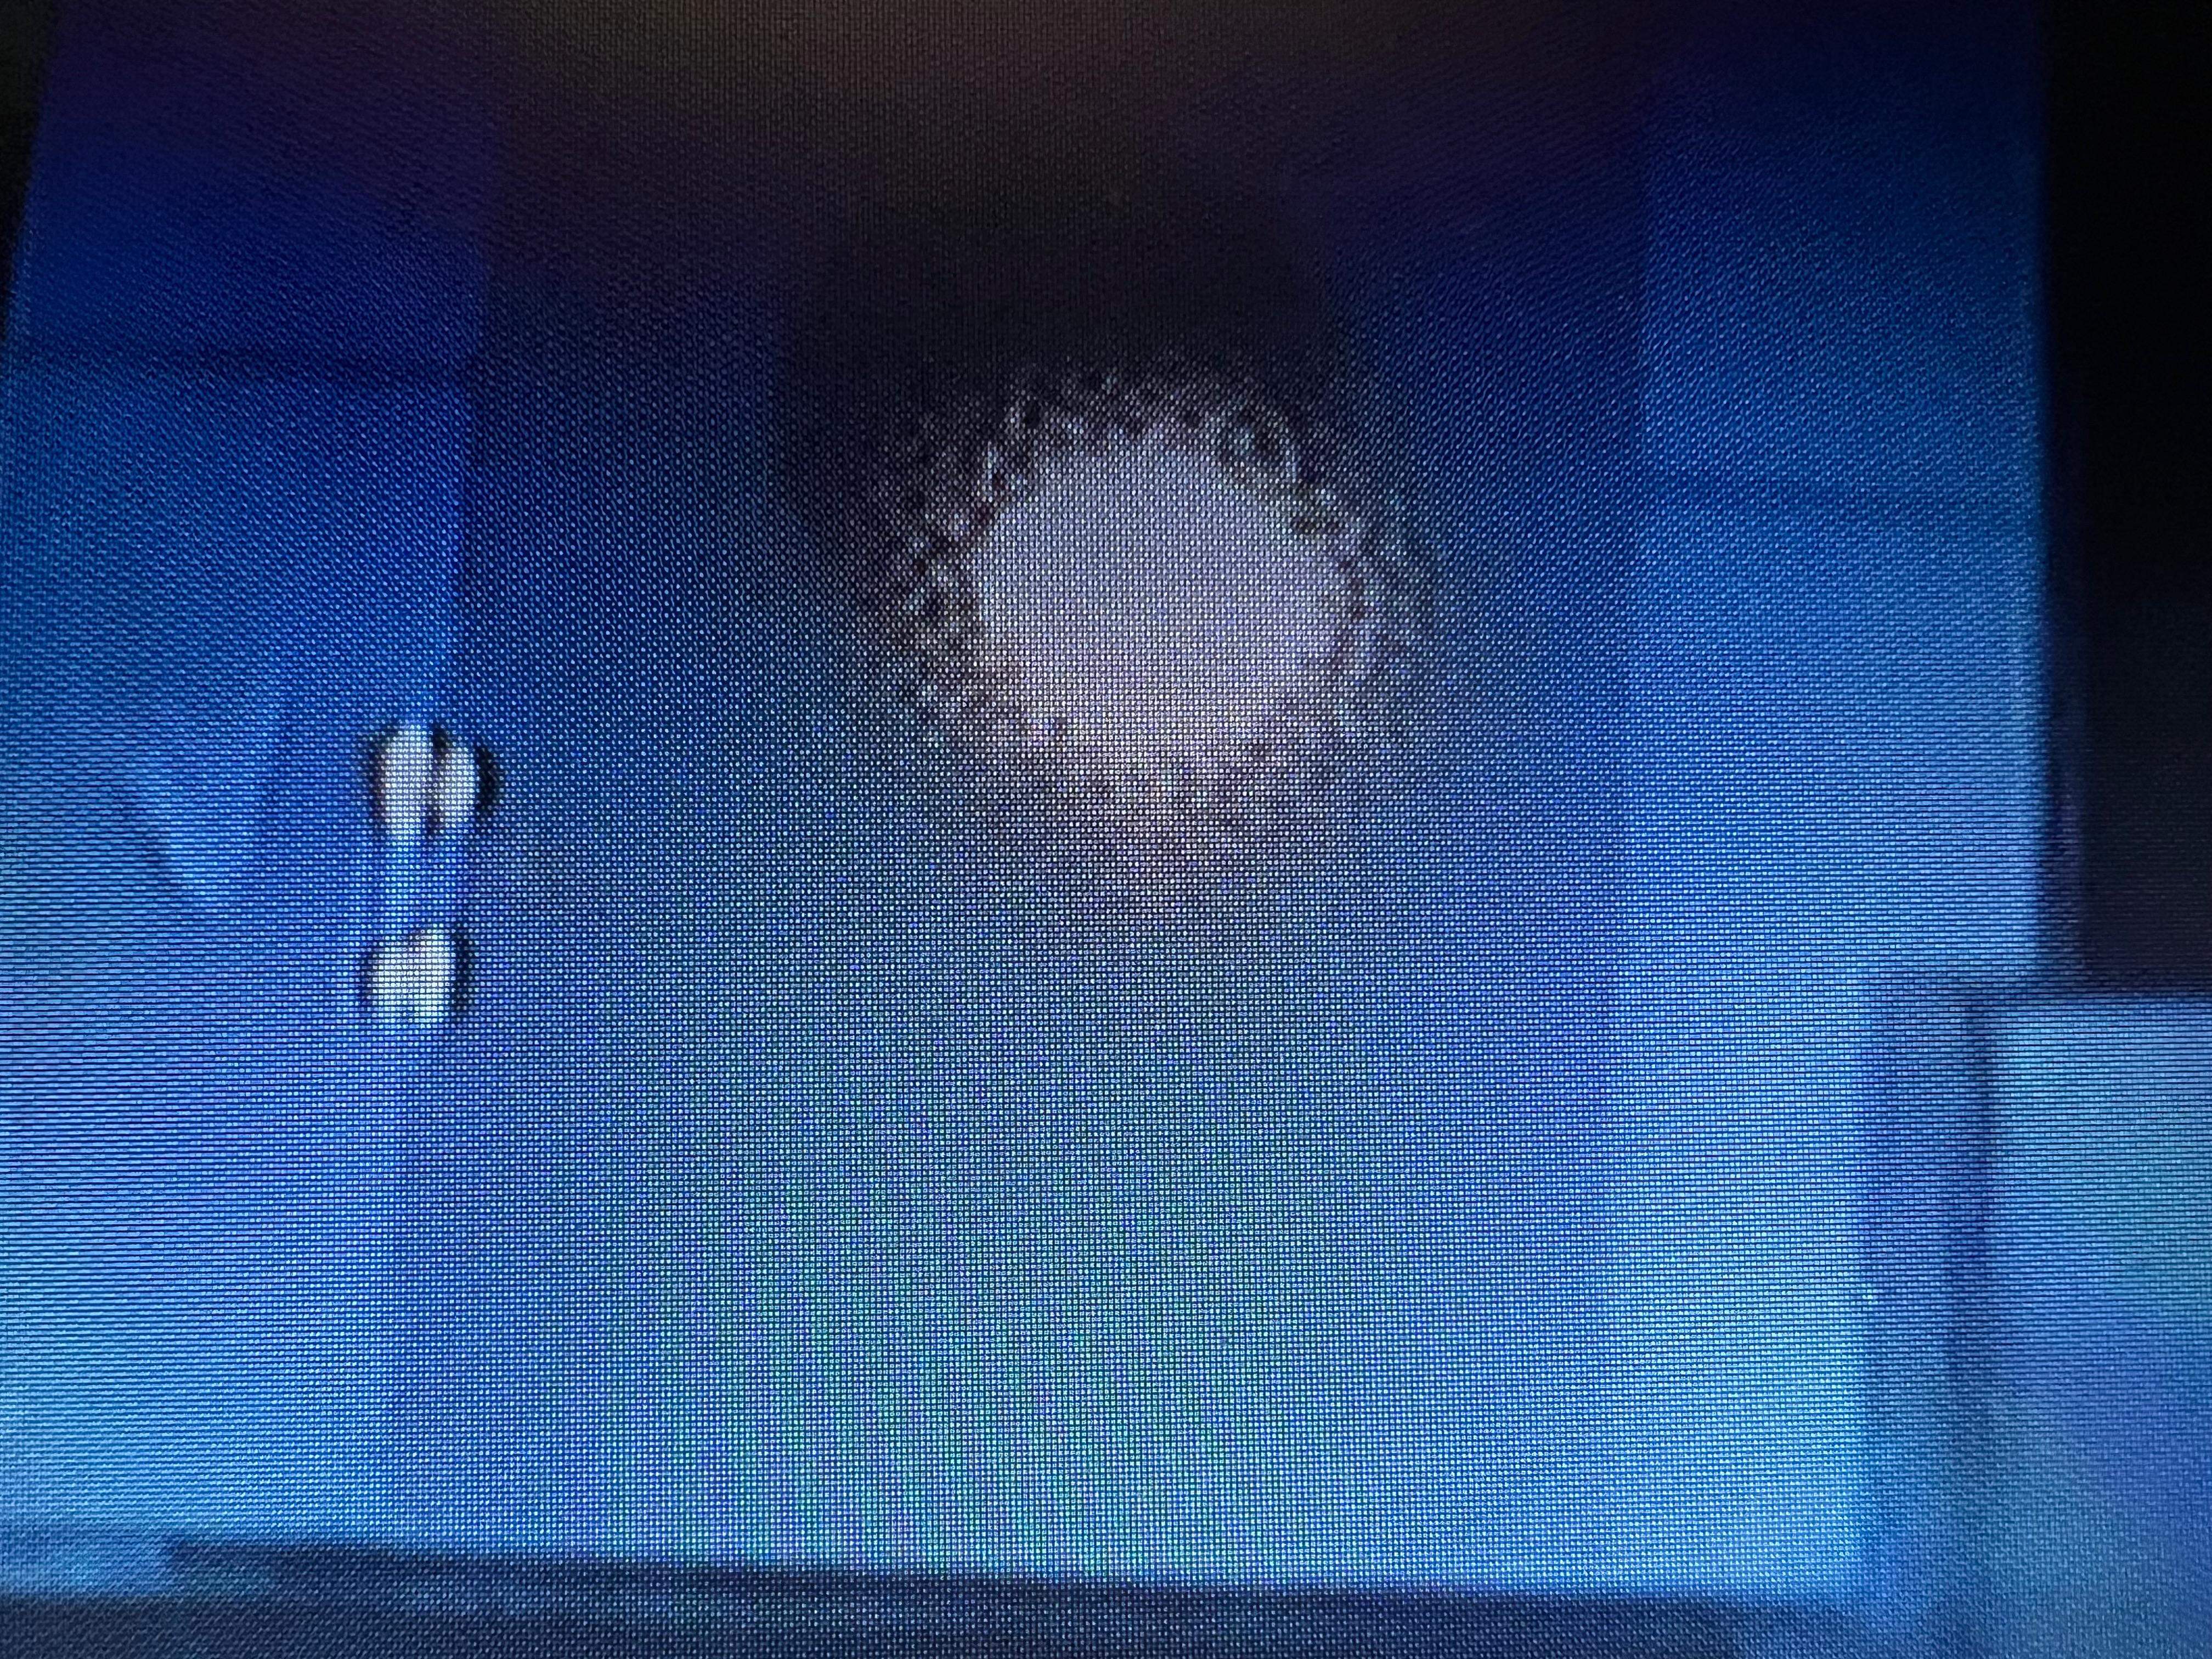
\includegraphics[width=0.5\textwidth]{content/images/lasingphase.jpeg}
  \caption{Deutliche Lasingaktivität auf der IR-Sichtkarte.}
  \label{fig::lasingphase}
\end{figure}

\begin{table}
  \centering
  \caption{Eine Beispieltabelle mit Messdaten.}
  \label{tab:tabelle}
  \sisetup{table-format=1.1, per-mode=reciprocal}
  \begin{tblr}{
      colspec = {S[table-format=3.0] S[table-format=2.1] S},
      row{1} = {guard, mode=math},
      vline{4} = {2}{-}{text=\clap{$\pm$}},
    }
    \toprule
    U \mathbin{/} \unit{\volt} & I \mathbin{/} \unit{\micro\ampere} & \SetCell[c=2]{c} N \mathbin{/} \unit{\per\second} & \\
    \midrule
    360 & 0.1 & 98.3 & 0.9 \\
    400 & 0.2 & 99.8 & 1.0 \\
    420 & 0.2 & 99.1 & 0.9 \\
    \bottomrule
  \end{tblr}
\end{table}

Siehe \autoref{fig:plot} und \autoref{tab:tabelle}!
